Over the course of this chapter, the design of the communication protocol in all variants will be thorougly explained. To begin, fundamental
assumptions about the environment and basic building blocks of the protocol are presented. Since the protocol variants share many elements and differ
mostly in the authentication scheme and the application of network coding, the simplest one (uncoded individual authentication) is used to give a
step-by-step explanation of the full protocol. Following this, the other variants are described by drawing upon the differences to uncoded individual
authentication. Finally, the routing strategies that are explored in conjunction with the protocol are elaborated.

\section{Design Aspects}
\subsection{Unicast And Multicast}
In Section \ref{sec:assandsig}, it was already hinted that this thesis concerns itself with the unicast communication pattern. In this scenario, each
flit is sent to a single specified destination. In contast, multicast facilitates the existance of multiple receivers for a single flit.

While there has been notable work on \gls{noc} multicast protocols, especially in conjuction with network coding, this thesis builds directly upon
research in the unicast domain (cf. Section \ref{sec:ncfornoc}). Hence, multicast will not be considered for the implementation, experiments, and
evaluation performed here.

\subsection{Flit Structure}\label{subsec:flitstructure}
As mentioned in Section \ref{sec:flitsfun}, flits are the fundamental unit of transmission for this thesis. They contain several header fields and a
payload. Their structure differs slightly depending on whether or not network coding is employed. For network coded flits, one additional
header field is required (the global encoding vector) and the generation ID replaces the flit ID. This structure is depicted in Figure
\vref{fig:flitstructureuncoded} (uncoded) and Figure \ref{fig:flitstructurenetworkcoded} (network coded).
% TODO: table comparing the protocol variants, their properties (e.g. lane width)

\begin{figure}
    \centering
    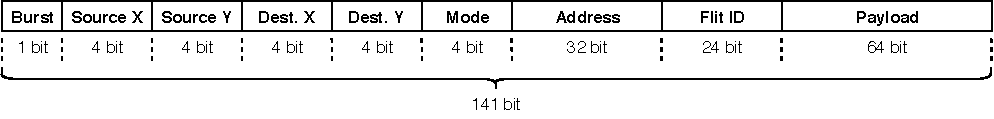
\includegraphics[width=\textwidth]{flit-structure-uc}
    \caption[The structure of a flit without network coding]{The structure and data layout of a flit in an environment without network coding
    (uncoded). The fixed size of the header fields and the payload results in an invariant total size of 141 bit.}
    \label{fig:flitstructureuncoded}
\end{figure}

\begin{figure}
    \centering
    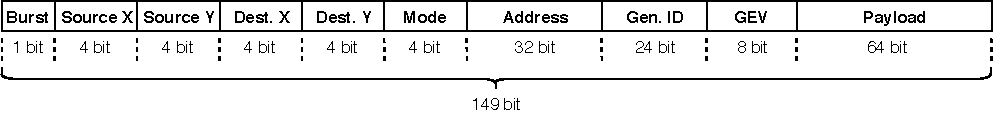
\includegraphics[width=\textwidth]{flit-structure-nc}
    \caption[The structure of a flit with network coding]{The structure and data layout of a flit in a network coded environment. The fixed size of
    the header fields and the payload results in an invariant total size of 149 bit.}
    \label{fig:flitstructurenetworkcoded}
\end{figure}

The header fields are required for routing the flits to their destinations and for correct processing by the receivers, while the payload carries the
transmitted information. Uncoded flits have the following fields:
\begin{itemize}
    \item \textbf{Burst.} The burst bit is used to indicate an uninterrupted stream of flits between the same sender and receiver. For example, when a
        larger packet is being broken down into multiple flits, the burst bit can be used to indicate the beginning of a flit stream, allowing the
        intermediate routers on the path to the receiver to adjust their routing behavior accordingly in order to minimize stream interruptions. In
        this thesis, however, the burst bit is unused. As there are plans to build upon this work and explore burst configurations, it is included
        nevertheless for documentation purposes.
    \item \textbf{Source X, Source Y.} Recalling that the topology of the \gls{noc} is a 2D mesh, the usage of 2D cartesian coordinates to uniquely
        identify nodes suggested itself. Here, zero-based X and Y indices indicate the column and row of a node, respectively. Each field is 4 bit long,
        resulting in at most $16 \cdot 16 = 256$ nodes being addressable. Hence, the maximum \gls{noc} size is \textit{16x16} as well, which is deemed
        sufficient\footnote{It is certainly possible to increase the field sizes to, e.g., 8 bit, allowing for up to $256 \cdot 256 = 65536$ addressable
        nodes, should the need arise. However, as this would increase the flit size, it is not implemented here.}. The source header fields describe
        the address of the flit's sender.% TODO: refer to a figure describing a routing strategy, which shows addresses of a sender and receiver
    \item \textbf{Destination X, Destination Y.} These fields also describe the address of a node in 2D cartesian coordinates. As opposed to the
        source fields, they indicate the intended destination of the flit.
    \item \textbf{Mode.} The mode field indicates what type of data the flit contains. It signals to the receiver whether the flit contains, e.g.,
        data, a \gls{mac}, or an \gls{arq}. There are a few more special modes that are explained in Section \ref{sec:theprotocol}. The
        field size is 4 bit, allowing for 16 different modes. Not all of them are used for this thesis, so it is possible to define additional modes
        in a future work if necessary.
    \item \textbf{Address.} This field may contain a 32 bit memory address. In case the flit payload needs to be read from or written to memory, it
        indicates the location of the data. Since this is only relevant to the processing elements and not the network interfaces, the field remains
        unused for this thesis. Nevertheless, it is included in the flits since it affects their size.
    \item \textbf{Flit ID.} The flit ID is a 24 bit numeric identifier. Starting at zero, the IDs are incremented as more flits are generated.
        Similar to sequence numbers (e.g., as employed in \gls{tcp}), they are used to ensure that all flits arrive at the destined processing
        elements in order. Furthermore, the values are used to associate related flits. For instance, an encrypted data flit and the corresponding \gls{mac}
        flit have the same ID to express their correlation.
    \item \textbf{Payload.} The payload carries the actual data that are transmitted with a flit. Its size is 64 bit as this is a common block size
        for ciphers, such as the one used for this thesis, PRINCE \cite{borghoff12prince}.
\end{itemize}
\vspace{0.5\baselineskip}

When network coding is applied to a flit, the following fields are added:
\begin{itemize}
    \item \textbf{Generation ID.} Replacing the flit ID, the generation ID is also a 24 bit numeric idenfier. As network coding intermingles multiple
        flits, their original IDs become meaningless and are replaced by the generation ID (which is the same for all flits of a generation). Apart
        from this, they follow the same rules as the flit IDs described above.
    \item \textbf{Global Encoding Vector.} This field contains the global encoding vector used to create the flit when applying network coding. It is
        required for the receiver to successfully decode a generation and obtain the original flits. Furthermore, since all flits in a generation have
        the same ID, it is used to distinguish between those flits. As with flit IDs in an uncoded setting, corresponding flits (like data and
        \gls{mac}) are associated by having the same \gls{gev} in addition to the same generation ID.
\end{itemize}
\vspace{0.5\baselineskip}

With a size of 141 or 149 bit, respectively, flits are relatively small. While this entails that each one carries comparatively little
information\footnote{The combined size of the header fields (77 or 85 bit, respectively) exceeds the size of the payload (64 bit) considerably.}, it
has the significant advantage that flits can be transferred between directly connected components in a single clock
cycle. For example, sending a flit from a router to a neighboring one, or sending it from a processing element
to the attached network interface takes one cycle. In a hardware implementation, this is facilitated by parallel communication channels that are able
to transmit multiple bits simultaneously. This results in multiple wires (or other electical conductors) at the physical layer, as each one may convey
precisely one bit of information per cycle \cite{wikiparallelcomm}. Thus, for uncoded flits, a channel width of 141 or more wires is required, and at least 149
in a network coded setting.

\subsection{Cryptography}\label{subsec:crypto}
\subsubsection{Notation}\label{subsubsec:cryptonotation}
This section introduces formal notations and definitions regarding the cryptographic primitives. They will be used throughout this chapter to
illustrate how flits are processed. They are denoted by variables, functions, and operators, where
\begin{itemize}
    \item $p$ is a plaintext message (which corresponds to the flit payload),
    \item $c$ is a ciphertext,
    \item $m$ is a \gls{mac},
    \item $k$ is a key (with $k_e$ and $k_m$ referring to encryption and \gls{mac} keys),
    \item $f$ is a complete flit (header and payload),
    \item $r$ is an authenticated and encrypted message,
    \item $e_k(p)$ is an encryption function that takes a plaintext $p$ and produces a ciphertext $c$ using key $k$ (sometimes denoted by a lock
        symbol),
    \item $d_k(c)$ is a decryption function that takes a ciphertext $c$ and produces the plaintext $p$ using key $k$,
    \item $a_k(f)$ is an authentication function that takes a flit and produces a \gls{mac} $m$ using key $k$\footnote{The whole flit is
        authenticated, as opposed to just the payload, to provide integrity on the header fields as well.},
    \item $\oplus$ denotes the bitwise XOR operation, and
    \item $\|$ symbolizes concatenation.
\end{itemize}
\vspace{0.5\baselineskip}

While the functions $e_k(p)$ and $d_k(c)$ take a 64 bit long text as their argument (which matches the cipher's block size), the authentication
function $a_k(f)$ is applied to complete flits, exceeding the block size. Therefore, $a_k(f)$ applies the cipher in conjunction with the \gls{cbcmac}
mode of operation as explained below.

\subsubsection{Drawbacks}\label{subsubsec:cryptodrawbacks}
The integration of cryptographic operations inevitably entails a degradation of the network performance which manifests itself in higher transmission
latencies and increased chip area requirements. There usually is a reversely proportional relation between performance and safety: as the level of security
increases, the communication performance declines. In order to satisfy the protection goals of confidentiality and integrity, both encryption and
authentication are required\footnote{Depending on the use case, it may be adequate to fulfill only one of these goals (or none at all), alleviating
the performance drop caused by the security measures. For instance, a preceding work of this thesis concerns itself with providing only integrity in
\glspl{noc} \cite{moriam18activeattackers}.}, resulting in a noticeable performance impact. In order to minimize these effects, several countermeasures
are implemented:
\begin{itemize}
    \item \textbf{Parallel modules.} As the cryptographic computations are the operations with the highest latency in the network interfaces, they
        threaten to become a bottleneck and congest the traffic flow. To prevent this, multiple cryptographic modules are employed in each network
        interface. While this does not speed up the individual cryptographic computations, it allows for multiple flits to be processed in parallel. For
        instance, each network interface could have three encryption modules, allowing it to encrypt up to three flits simultaneously. Alas, this
        approach naturally increases the occupied chip area.
    \item \textbf{Hardware-optimized ciphers.} In Section \ref{sec:lightweightcrypto}, it was already mentioned that conventional block ciphers, such
        as \gls{aes}, are not efficient enough for usage in \glspl{noc}, in terms of both latency and chip area. However, there is a plethora of
        algorithms specifically designed for an efficient hardware implementation. In the work directly preceding this thesis, they were evaluated and
        compared \cite{harttung17lightweightcrypto}. The most promising algorithm is PRINCE \cite{borghoff12prince}, which is introduced below.
    \item \textbf{Parallel decryption and verification.} When flits arrive from the network, the \gls{mac} is verified to ensure integrity. When
        successful, the data are decrypted and passed on. To speed up this process, verification and decryption is performed in parallel. Should the
        integrity check fail, the decrypted data have to be discarded. In case of success, however, this results in a significant latency reduction.
        This scheme is illustrated in detail in the step-by-step description of the protocol (Section \ref{sec:theprotocol}).
\end{itemize}

\subsubsection{Composition Methods}
The ordering of encryption and authentication (i.e., \gls{mac} computation) has a significant impact on both the achievable performance and the
security of the scheme. There are three general approaches to bring them together \cite{bellare00authenc}:
\begin{itemize}
    \item \textbf{Encrypt-and-MAC (\gls{eam}).} The plaintext is encrypted and the \gls{mac} is computed over the plaintext. Afterwards, the \gls{mac} is
        appended to the ciphertext. More precisely, $r = e_{k_e}(p)\|a_{k_m}(f)$.
    \item \textbf{MAC-then-Encrypt (\gls{mte}).} The \gls{mac} is computed over the plaintext and then appended to it. The result is then
        encrypted. In other words, $r = e_{k_e}(p\|a_{k_m}(f))$.
    \item \textbf{Encrypt-then-MAC (\gls{etm}).} First, the plaintext is encrypted. Subsequently, the \gls{mac} is computed over the ciphertext and appended to it.
        Namely, $c = e_{k_e}(p)$ and $r = c\|a_{k_m}(f_c)$ where $f_c$ refers to the flit with encrypted payload.
\end{itemize}
\vspace{0.5\baselineskip}

Out of these three methods, \gls{etm} was chosen. It provides integrity on the ciphertext -- and consequently on the plaintext as well --
instead of just the plaintext. Thus, the integrity of the message can be verified without the need to decrypt it first and the parallel decryption and
verification mentioned above becomes possible. Moreover, in case of an integrity breach, \glspl{arq} can be issued earliest as the verification is
performed directly after the flits arrive.

On the sender side, \gls{etm} necessitates sequential encryption and authentication since the \gls{mac} is computed over the ciphertext. While
\gls{mte} forces this as well, it can be parallelized with \gls{eam}. However, both \gls{eam} and \gls{mte} do not provide an overall speed gain over
\gls{etm}. In addition, they have been subject to security vulnerabilities in the past \cites{bellare00authenc}{bellare04ssheam}{etmtls}. Table
\ref{tab:compositionmethods} gives a comparison of the methods.

\begin{table}
    \centering
    \begin{tabulary}{\textwidth}{L|CCC}
        & \gls{eam} & \gls{mte} & \gls{etm} \\\hline
        Parallel encryption/authentication & yes & no & no \\
        Parallel decryption/verification & no & no & yes \\
        Plaintext integrity & yes & yes & yes \\
        Ciphertext integrity & no & no & yes \\ % TODO: more aspects?
        Verification latency & high & high & low
    \end{tabulary}
    \caption[Comparison of authenticated encryption composition methods]{Comparison of the authenticated encryption composition methods
    Encrypt-and-MAC (\gls{eam}, MAC-then-Encrypt (\gls{mte}), and Encrypt-then-MAC (\gls{etm}).}
    \label{tab:compositionmethods}
\end{table}

For all methods, the ciphertext and \gls{mac} need to be embedded into one or more flits since they cannot be sent without the header fields. This is
elucidated in the protocol descriptions (Section \ref{sec:theprotocol}).

\subsubsection{PRINCE}\label{subsubsec:prince}
The cipher that is used for encryption, decryption, and authentication is \textit{PRINCE} \cite{borghoff12prince}. Among its many competitors, it is
the algorithm of choice because it has the lowest encryption and decryption latency with a competitive area requirement
\cite{harttung17lightweightcrypto}. Here, low latency is deemed more important than low chip area requirements, rendering it a natural choice. Besides, the
faster the algorithm runs, the less parallel modules may be required, potentialls reducing the overall area requirement in the end. Furthermore, with a
key length of 128 bit, it provides relatively high security\footnote{Similar algorithms often have a key length of just 80 or 96 bit
\cite[5]{harttung17lightweightcrypto}.}. To date, it remains unbroken despite monetary incentives to develop attacks \cite{princechallenge}.

PRINCE is a symmetric block cipher with a block size of 64 bit and a key size of 128 bit. It is structured as a \textit{substitution-permutation
network (\gls{spn})} with 12 rounds.

What sets PRINCE apart from other lightweight ciphers is a design specifically targeted at fully unrolled hardware implementations. With this
strategy, each round is computed using its own dedicated part of the circuit. These pieces are concatenated to form the full cipher. This approach
enables the algorithm to be executed within a single clock cycle. In contast, traditional iterative implementations of round-based ciphers usually
have a single circuit constituting the round function that is reused for all rounds. There, one clock cycle per round is required.

Although single-cycle execution suggests a tremendously low latency, the number of cycles cannot be directly mapped to execution speed. The long critical path
entailed by the chained round functions results in a relatively low maximum clock frequency. Furthermore, the unrolled design entails a comparatively
higher area requirement than iterative ones; however, it is still \enquote{considerably lower than fully unrolled versions of \gls{aes} or PRESENT}
\cite[3]{borghoff12prince}.

The authors of PRINCE have investigated the maximum clock frequency of their algorithm under varying conditions. They were able to achieve 212.8 MHz
using speed-optimizing synthesis strategies and 45 nm technology\footnote{Their other tests include 90 and 130 nm technology or area-optimizing
synthesis strategies, yielding lower results.}. In other research \glspl{noc} at the TU Dresden, namely the \textit{Tomahawk}
\gls{mpsoc}, 28 nm technology is commonly used \cite[35]{cfaedreport}. Under
this premise, a frequency of at least 250 MHz is definitely achievable, considering that the switch from 90 to 45 nm already more than doubled
the maximum frequency in the authors' experiments.

A great asset of PRINCE is the possibility to use almost the exact same algorithm for encryption and decryption. More precisely, the decryption
function corresponds to the encryption function if the round key\footnote{PRINCE uses the same round key for all rounds.} for the former is slightly
modified. At the start of PRINCE, three subkeys $(k_0, k_0', k_1)$ are derived from the main key $k$, with $k_1$ being the round key\footnote{The
other keys, $k_0$ and $k_0'$ are used as whitening keys.}. Now, $d_{(k_0, k_0', k_1)}(c) = e_{(k_0, k_0', k_1 \oplus \alpha)}(c)$, where $\alpha$ is a
64 bit constant. This property, called \textit{\alpha-reflection}, renders using the same circuit for encryption and decryption possible by simply
omitting the XOR operation for the encryption case.

\subsubsection{A Note On Stream Ciphers}
While block ciphers dominate the lightweight cryptography field of research, there has been notable research on stream ciphers as well
\cite[cf.][]{estream}. In terms of speed and size, they sometimes even surpass block ciphers. For example, the stream cipher \textit{Trivium}
\cite{decanniere06trivium} is smaller than PRINCE and also able to encrypt up to 64 bit in one clock cycle \cite[8]{harttung17lightweightcrypto}.

The reason stream ciphers were ultimately not considered for this thesis is twofold. First, they require keeping an internal state from which the
keystream is derived (288 bit for Trivium). As each node pair uses its own shared secret key, all nodes would need to keep such state information for
every other node in the network, necessitating large buffers. Second, in comparison to block ciphers, stream ciphers have been studied very little,
potentially increasing the risk of security flaws in this construction technique.

\subsection{Random Linear Network Coding}\label{sec:designnc}
The coding scheme used in this work is a variant of \textit{Random Linear Network Coding (\gls{rlnc})} and based on the work of
\citeauthor{moriam15manycorenc} \cite{moriam15manycorenc}. It slightly differs from the traditional idea of network coding
\cites{ahlswede00networkflow}{li03linearnc}. First, the targeted communication pattern is not multicast, but unicast transmissions, since only the
latter are of interest for this thesis. Second, only the sender nodes compute combinations of flits (intermediate nodes merely forward them) and only
flits with the same destination are coalesced (\enquote{intra-session network coding} \cite[1]{moriam15manycorenc}). The rationale behind this are the
tight performance requirements of the \gls{noc}. If each network node were to buffer incoming flits until enough are present to perform local
encoding, routing latencies would increase considerably. Furthermore, the implementation of local encoding necessitates additional memory and
processing logic inside each router, making their design more complex and increasing their size. As this directly contradicts the \gls{noc} design goals
laid out in Section \ref{sec:networkonchipfun}, it is not considered here.

\subsubsection{Operation Breakdown}
In the implemented approach, the sender organizes flits $f_i\ |\ i \in \mathbb{N}, i = 0, …, n$ with the same destination into generations $g_j\ |\ j
\in \mathbb{N}, j = 0, …, \lfloor\frac{n}{2}\rfloor$ of size $G$. Here, each generation consists of 2 flits (i.e., $G = 2$)\footnote{Larger
generations, consisting of three or more flits, are also feasible, but have proven to entail higher transmission latencies \cite[2]{moriam18activeattackers}, which
is not desirable.} and is constructed as $g_j = (f_{2j}, f_{2j+1})$. Furthermore, the flit IDs $i$ are replaced in the flits by the generation IDs $j$
as described in Section \ref{subsec:flitstructure} (see also Figure \vref{fig:encodingexample}).

The combinations are then computed as follows: first, a unit vector $e_i = (e_{i_0}, …, e_{i_{G-1}})$ that signifies the index of the flit inside the
generation \cite[cf.][3]{chou03practicalnc} is prepended to each flit's payload:
\[
    e_{i_k} =
    \begin{cases}
        1 & |\ i = k \pmod G \\
        0 & |\ i \neq k \pmod G
    \end{cases}
\]
These vectors and the payloads are then organized as a matrix for each generation:
\[
    \begin{split}
        \begin{bmatrix}
            e_{0,\,0} & \cdots & e_{0,\,G-1} & p_{0,\,0} & \cdots & p_{0,\,P-1} \\
            \vdots & \ddots & \vdots & \vdots & \ddots & \vdots \\
            e_{G-1,\,0} & \cdots & e_{G-1,\,G-1} & p_{G-1,\,0} & \cdots & p_{G-1,\,P-1}
        \end{bmatrix}\\
        =
        \begin{bmatrix}
            1 & & 0 & p_{0,\,0} & \cdots & p_{0,\,P-1} \\
            & \ddots & & \vdots & \ddots & \vdots \\
            0 & & 1 & p_{G-1,\,0} & \cdots & p_{G-1,\,P-1}
        \end{bmatrix}
    \end{split}
\]
where $P$ corresponds to the payload size in symbols. Network coding is performed in $GF(2^4)$ as this entails a sufficiently high invertibility
probability of the coefficient matrix and relatively small \glspl{gev} (see below for details). Thus, the symbol size is 4 bit and $P = 16$. Now,
$C \geq G$ combinations are computed with randomly selected coefficients $\beta$ \cite[cf.][]{ho03randomcoding}:
\[
    \begin{split}
        \begin{bmatrix}
            \beta_{0,\,0} & \cdots & \beta_{0,\,G-1} & q_{0,\,0} & \cdots & q_{0,\,P-1} \\
            \vdots & \ddots & \vdots & \vdots & \ddots & \vdots \\
            \beta_{C-1,\,0} & \cdots & \beta_{C-1,\,G-1} & q_{C-1,\,0} & \cdots & q_{C-1,\,P-1}
        \end{bmatrix}\\
        =
        \begin{bmatrix}
            \beta_{0,\,0} & \cdots & \beta_{0,\,G-1}\\
            \vdots & \ddots & \vdots \\
            \beta_{C-1,\,0} & \cdots & \beta_{C-1,\,G-1}
        \end{bmatrix}
        \begin{bmatrix}
            1 & & 0 & p_{0,\,0} & \cdots & p_{0,\,P-1} \\
            & \ddots & & \vdots & \ddots & \vdots \\
            0 & & 1 & p_{G-1,\,0} & \cdots & p_{G-1,\,P-1}
        \end{bmatrix}
    \end{split}
\]
Each row of the result matrix represents one combination, with $\beta_i = (\beta_{i,\,0}, …, \beta_{i,\,G-1})\ |\ i \in \left[0, C\right)$ standing
for the \glspl{gev} and $q_i = (q_{i,\,0}, …, q_{i,\,P-1})\ |\ i \in \left[0, C\right)$ corresponding to the encoded payloads. The other header fields
are adopted unaltered from the original flits\footnote{The header fields of the original flits in the same generation contain the same values by
design, hence these values can simply be copied to the encoded flits.}. Figure \vref{fig:encodingexample} illustrates the whole process.

\begin{figure}
    \centering
    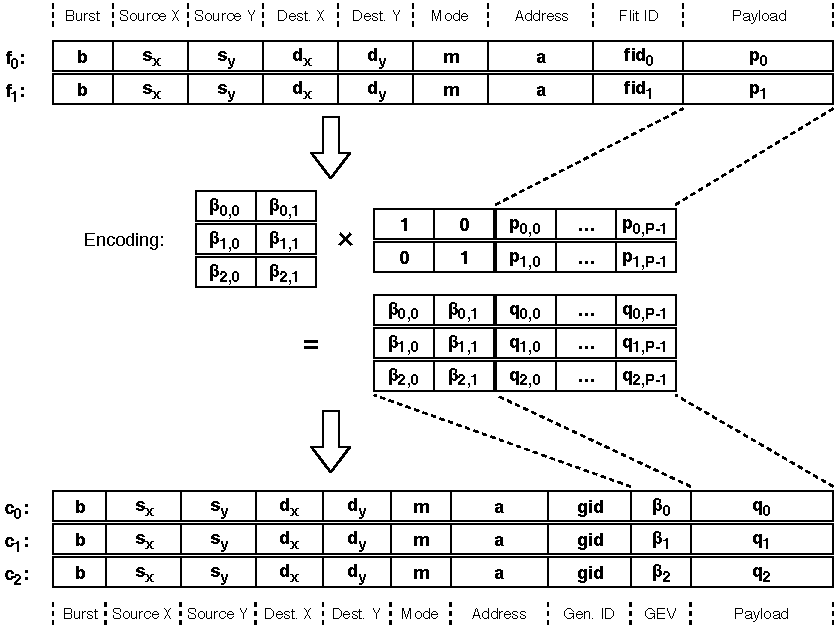
\includegraphics[width=\textwidth]{encoding-example-mapping}
    \caption[Application of network coding to flits]{Application of network coding to flits. The generation size is G=2 and the number of computed
    combinations is C=3 (i.e., the G2C3 scheme). Using randomly selected cofficients $\beta$ as \glspl{gev}, the flits $f_0$ and $f_1$ are encoded,
    creating the combinations $c_0$, $c_1$, and $c_2$.}
    \label{fig:encodingexample}
\end{figure}

For this thesis, variants with $C = 3$ and $C = 4$ combinations per generation are investigated \cite[cf.][2]{moriam18activeattackers}. These schemes
are referred to as \textit{G2C3} and \textit{G2C4}, respectively.

On the side of the receiver, the combinations\footnote{Henceforth, the term \textit{combination} is also used to refer to the flit containing a
combination.} are decoded to recover the original flits. At least $G$ out of the $C$ combinations must arrive at their
destination to render decoding possible. Furthermore, the $G$ combinations have to be linearly independent. With a symbol size of 4 bit and randomly
selected coefficients, they fulfill this condition with a probability of $\approx 93\%$ \cite[4]{franz18authdraft}\footnote{A larger symbol size would
entail higher invertibility probabilities. For example, it is $>99\%$ for a symbol size of 8 bit \cite[4]{franz18authdraft}, but at the cost of the
\gls{gev} size being doubled. Hence, 4 bit are deemed sufficient for this thesis.}. Should this condition be violated, a different set of $G$ out of
the $C$ combinations is used\footnote{In the rare case that decoding is unsuccessful for any $G$ of the $C$ combinations, this generation cannot be
recovered. For the remainder of this thesis, it is assumed that the combinations are always linearly independent for simplicity.}. The receiver then
decodes the combinations by solving the system of linear equations established by the received flits' \glspl{gev} and payloads:
\[
    \begin{bmatrix}
        \beta_{0,\,0} & \cdots & \beta_{0,\,G-1} & q_{0,\,0} & \cdots & q_{0,\,P-1} \\
        \vdots & \ddots & \vdots & \vdots & \ddots & \vdots \\
        \beta_{G-1,\,0} & \cdots & \beta_{G-1,\,G-1} & q_{G-1,\,0} & \cdots & q_{G-1,\,P-1}
    \end{bmatrix}
\]
The solution is obtained by applying Gaussian elimination until the matrix is in reduced row echelon form with the following structure:
\[
    \begin{bmatrix}
        1 & & 0 & p_{0,\,0} & \cdots & p_{0,\,P-1} \\
        & \ddots & & \vdots & \ddots & \vdots \\
        0 & & 1 & p_{G-1,\,0} & \cdots & p_{G-1,\,P-1}
    \end{bmatrix}
\]
Now, the original flits may be recreated. The vectors $p_i = (p_{i,\,0}, …, p_{i,\,P-1})\ |\ i \in \left[0, G\right)$ obtained from the system of linear
equations above are their payloads. The flit IDs are reconstructed from the generation ID $j$: with $G = 2$, they are $2j$ and $2j+1$. The other
header fields are simply copied over from one of the combinations as they have not changed during the encoding phase.
% TODO: vector symbols over p_i, beta_i etc. where appropriate (im Fließtext)

\subsubsection{Effect On The Network}
On the one hand, \gls{rlnc} provides the great benefit that flit loss is tolerable to a certain degree. If $C > G$, i.e., the number of computed
combinations per generation is greater than the generation size, then flawless decoding is still possible for the receiver when up to $C - G$ flits
are lost in transit.

On the other hand, the amount of flits injected into the network increases considerably depending on the coding scheme. For G2C3, 50\% more flits are
sent out, and 100\% more for G2C4 (compared to uncoded communication). However, the additional resilience to flit loss entails less \glspl{arq} to be
issued (in an unreliable network), which in turn may reduce the overall load.

\subsection{Flit And Generation IDs}
For each sender-receiver pair, the IDs of flits and generations should be unique in order to eliminate ambiguities between flits and inhibit replay
attacks. Hence, IDs start at zero and are incremented with each newly created flit or generation, respectively. However, as only a finite amount of
distinct values can be represented by the carrying header field, long-running systems are bound to cause an arithmetic overflow at some point. Prior
to this thesis, a size of 24 bit was determined as sufficient for the given scenario \cite[5]{franz18authdraft}. With this, $2^{24} = \num{16777216}$
distinct IDs are at disposal. Should an overflow occur, the IDs simply restart at zero. At this point, is is advisable to negotiate a new shared
secret key with the affected receiver to further impede replay attacks. For the remainder of this thesis, IDs are assumed to be unique for a given
sender-receiver pair.
% TODO: correct biblatex entry for the draft paper

\subsection{Transmission Units}
The concept of transmission units spans all protocol variants. In general, it signifies a group of flits belonging together, which is indicated by
having the same ID. For uncoded protocol versions, data flit and corresponding \gls{mac} flit (individual authentication) or first and second half of a
split (interwoven authentication) belong to the same transmission unit. With network coding, it corresponds to the generations; it is used to refer to
the set of combinations created from one generation together with any \glspl{mac} flits computed for these combinations.

\subsection{Retransmissions}\label{subsec:arqretransmissions}
As introduced in Section \ref{sec:reliability}, \glspl{arq} are used to request the retransmission of specific flits in the event of a loss or
corruption in transit. \Glspl{arq} are special flits that receivers can send back to the originator of the affected transmission unit. Their structure
is identical to that of normal flits so that the routers do not need to distinguish between \glspl{arq} and other flits. The mode field is always set
to \textit{\gls{arq}} to differentiate them. However, the following header fields are of no use in \gls{arq} flits and are thus ignored (cf. Section
\ref{subsec:flitstructure}):
\begin{itemize}
    \item \textbf{Burst.} The burst bit is useless for \gls{arq} flits since they are always sent as individual entities and not as part of a stream.
        For this thesis, this is no different to normal flits as the burst bit is entirely unused anyway; nevertheless, it may be relevant to future
        experiments.
    \item \textbf{Global Encoding Vector.} Network coding is never applied to an \gls{arq} flit; it is always uncoded. Hence, there is no \gls{gev}
        associated with it. For the uncoded protocol variants, this fields does not even exist in the first place.
\end{itemize}
\vspace{0.5\baselineskip}

An \gls{arq} is always associated with the transmission unit that was unsuccessfully communicated. For uncoded protocol versions, the ID field
matches the flit ID of the affected unit; for network coded variants, it contains the same generation ID. However, it is desirable that the issuer of the
\gls{arq} can specify the precise flits that need to be retransmitted from this unit. To indicate this, the payload field is used. For uncoded
protocol versions, it contains a list of modes (i.e., the same values that are used for the mode header field) that specify the required flits. The
\gls{arq}'s ID together with the mode values suffice to uniquely identify the flits in question\footnote{To be precise, it uniquely identifies the flits
for the given sender-receiver pair.}. For the network coded protocol variants, the requested flits' \glspl{gev} are needed as well, so the \gls{arq}'s
payload contains a list of \gls{gev}/mode pairs instead. However, in the network coded case, not all \glspl{gev} are necessarily known to the issuer
since they are randomly selected by the sender of the original flits. For instance, only one flit from a generation might arrive at its destination
while the others are lost in transit. Then, the receiver would have to issue an \gls{arq} for all other flits while only knowing one \gls{gev}. In
such cases, the receiver issues an \gls{arq} as usual, but includes a list of \gls{gev}/mode pairs of those flits that have already arrived (i.e.,
the inverse of the default method). It is then the original sender's responsibility to retrieve and resend all except the specified flits\footnote{To
distinguish between \glspl{arq} specifying the missing/corrupted flits and \glspl{arq} specifying the received/intact flits, two different values for
the mode field exist that indicate an \gls{arq}. Depending on the type of \gls{arq}, the appropriate one is used.}. In the protocol descriptions
below, clarifying examples are included (Section \ref{sec:theprotocol}).

The payload field is not always large enough to carry all the required information. One \gls{gev}/mode pair is $8+4=12$ bit in size, allowing for up to
5 pairs to fit into the 64 bit payload. For example, with G2C4 and individual authentication, a transmission unit consists of the four combinations
and their four \gls{mac} flits, which exceeds the number of flits that may be specified within a single \gls{arq}. As a solution, special mode values
are introduced that represent multiple flits for the same \gls{gev} (e.g., both data and \gls{mac} flit). Thus, for the example above, only four
\gls{gev}/mode pairs are required at maximum (one for each \gls{gev} of the generation), totaling in $4\cdot(8+4)=48$ bit of information.

The number of allowed \glspl{arq} per transmission unit is limited to prevent network congestion. In the event that an \gls{arq} is required but the limit
was already reached, the transmission unit is considered a failure and no further attempt to recover is made.

When a particular network interface handles incoming flits from the network, there are two scenarios that trigger an \gls{arq} issuance. The first
case is an integrity check failing. The second case occurs when the temporal gap between the arrival of flits from the same transmission unit becomes
too large. As the first flit from a the unit arrives, a countdown timer is started that is associated with this unit. Upon receiving further flits
belonging to the same unit, the timer is reset. Should it reach zero (i.e., a timeout occurs), the remaining flits from this transmission unit are
assumed lost and an \gls{arq} is issued requesting their retransmission.

Once an \gls{arq} is issued, the countdown timer for the affected transmission unit is reset. However, it is set to a higher value than the
inter-arrival timeout described above. Moreover, this value depends on the Manhattan distance between the sender and receiver nodes in the network,
with a longer distance resulting in a higher timeout value. This is done to account for the round trip time of the \gls{arq} and its
answer. Details are discussed in Section \ref{subsec:arqtimeouts}.

It is desirable to send out as little \glspl{arq} as necessary to keep the network load as low as possible. Furthermore, with a limited
amount of \glspl{arq} available per transmission unit, care needs to be taken to not \enquote{waste} them too early. For instance, a timeout may
occur while a \gls{mac} is currently being computed for another flit from the same transmission unit. On the one hand, if an \gls{arq} is issued for
the missing flits immediately, but the integrity check for the received flits fails shortly after, an additional \gls{arq} may not be allowed due to
the limit, causing the whole unit to fail. On the other hand, postponing the \gls{arq} too long may cause unreasonable increases in latency. As a
middle ground, the issuance of \glspl{arq} is only postponed if other flits from the same transmission unit are currently being verified\footnote{More
precisely, a data flit is considered \enquote{currently being verified} if its corresponding \gls{mac} flit has already arrived from the network and
the verification \gls{mac} is currently being computed, i.e., obtaining the verification result is imminent.} in order to include those flits in the
\gls{arq} as well, should the integrity check fail.

\Glspl{arq} are not encrypted because they only contain metadata that are not confidential. Furthermore, they are not authenticated in order to save
time and trigger the retransmissions as quickly as possible. Unfortunately, with the integrity checks missing, malicious routers are able to undetectably
modify \gls{arq} flits. However, this does not open up additional avenues of attack. An adversary is always able to prevent the retransmissions
by simply dropping the \gls{arq} flit. Modifying the \gls{arq} to flood the network with false retransmissions is possible, but for a \gls{dos}
attack, the adversary could also generate a surge of flits itself; at worst, the strength of the attack would be amplified.

\section{The Protocol}\label{sec:theprotocol}
As mentioned in Section \ref{sec:protocolvariants}, three different communication schemes were envisioned, with the first two subdivided into uncoded
and network coded versions. The remainder of this section provides a comprehensive specification of all variants. The steps described are all
performed in the network interfaces.

\subsection{Individual Authentication}\label{subsec:indauth}
\subsubsection{Uncoded Variant}
This protocol variant, \textit{uncoded individual authentication}, is the simplest of the five schemes. Like all variants, it features encryption and
authentication of the data. Its name is derived from the way this is implemented: each data flit is individually authenticated and the \gls{mac} is
transmitted in a separate flit. A graphical overview from the outside is shown in Figure \vref{fig:protflitdistindauthuc}, while the internal steps for
both sending to and receiving from the network are given in Figure \vref{fig:protchartindauthuc}.

\begin{figure}
    \centering
    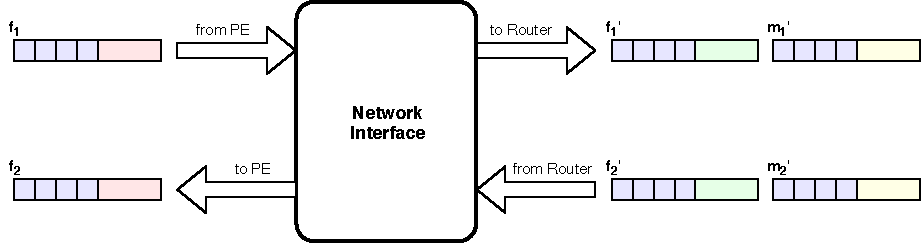
\includegraphics[width=\textwidth]{protocol-flit-distributions-indauth-uc}
    \caption[Uncoded ind. auth., outside view]{Outside view of the network interface for uncoded individual authentication. The processing of one
    transmission unit is depicted for both sending and receiving. For sending, the unencrypted flit $f_1$ results in the encrypted flit $f_1'$ and the
    corresponding \gls{mac} flit $m_1'$ being injected into the network. For receiving, the arrival of the encrypted flit $f_2'$ and its \gls{mac}
    $m_2'$ results in the decrypted flit $f_2$ being sent to the processing element.}
    \label{fig:protflitdistindauthuc}
\end{figure}

\begin{figure}
    \centering
    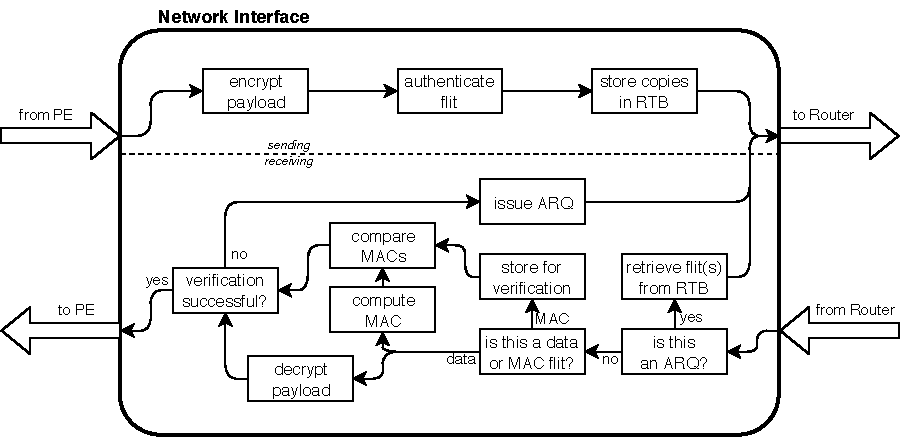
\includegraphics[width=\textwidth]{protocol-chart-indauth-uc}
    \caption[Uncoded ind. auth., detailed procedure]{The steps performed by the network interface when processing flits in the uncoded individual
    authentication protocol. The upper part of the chart illustrates the sending algorithm, while the lower part depicts the procedure for handling
    arrivals from the network.}
    \label{fig:protchartindauthuc}
\end{figure}

The sequence of actions for sending flits to the network (upper part of Figure \ref{fig:protchartindauthuc}) is as follows:
\begin{enumerate}
    \item \textbf{Encrypt payload.} For each flit arriving from the processing element, the payload is encrypted using the shared secret key of the
        flit's destination node. The employed cipher is PRINCE (see Section \ref{subsubsec:prince}). Since the payload length matches the cipher's
        block size (64 bit), one encryption operation suffices. All header fields remain untouched.
    \item \textbf{Authenticate flit.} The next part is to authenticate the encrypted flit. To achieve this, a \gls{mac} is computed over the entire
        flit, i.e., all header fields and the payload. Again, PRINCE is the cipher of choice. However, as the total size of the flit is 141 bit
        (exceeding the block size), a mode of operation is required to compute the \gls{mac}. Here, \gls{cbcmac} is employed\footnote{Standard
        \gls{cbcmac} is not secure for variable-length messages, where existential forgery is possible \cite{wikilengthextattack}. As the flits have a
        fixed length, this is not of concern here. However, an alternative algorithm such as \gls{cmac} could also be used.} because of its low
        complexity, resulting in a total of three required block encryptions. Since the last block would only contain 13 bit, it is
        padded (e.g., with zero-bits) to align it with the block boundaries. The computed \gls{mac} has a length of 64 bit. To transmit it, a new, dedicated
        \gls{mac} flit is created as follows: the mode field is set to \gls{mac}, the other header fields are copied from the data flit, and the
        \gls{mac} itself is inserted into the payload field\footnote{As data and \gls{mac} flit have the same ID, the receiver will be able to
        correctly link them together.}. Both flits are then sent out together. Figure \vref{fig:computeflitmac} elucidates this process.
    \item \textbf{Store copies in retransmission buffer.} Since \glspl{arq} may arrive to request retransmissions of already dispatched flits, the
        sender stores a copy of each flit in a dedicated retransmission buffer before sending it to the network. For each possible receiver,
        there is a separate buffer because the required storage time is proportional to the distance to the receiver. Thus, buffers for nodes far away are
        larger. Once a buffer is full, old flits are replaced in a \gls{fifo} manner\footnote{Naturally, the buffers should be large enough to be
        able to serve flits for \glspl{arq} arriving within an acceptable time frame after the original flit was dispatched. For simplicity, the
        buffers are assumed to be sufficiently large to handle all \glspl{arq}.}. The original flits are sent to the network.
\end{enumerate}
\vspace{0.5\baselineskip}

\begin{figure}
    \centering
    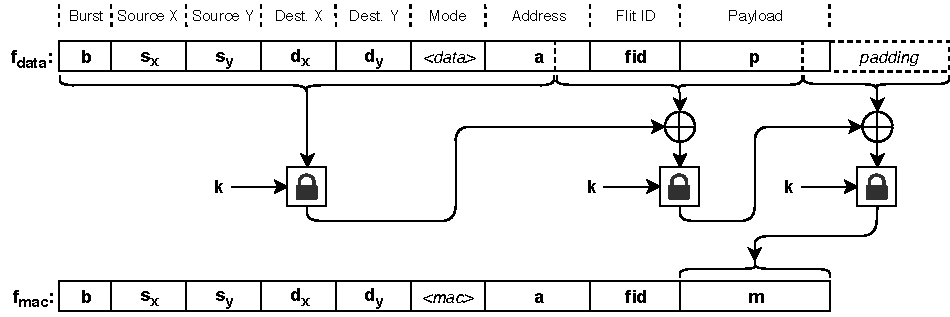
\includegraphics[width=\textwidth]{compute-flit-mac}
    \caption[CBC-MAC algorithm applied to an uncoded flit]{The \gls{cbcmac} algorithm applied to an uncoded flit. The flit is divided into three
    64-bit blocks, with the last one padded. Subsequently, a \gls{mac} is computed using \gls{cbcmac}, which is then inserted into the payload of a
    new flit.}
    \label{fig:computeflitmac}
\end{figure}

Arriving flits are processed via the following procedures (lower portion of Figure \ref{fig:protchartindauthuc}):
\begin{enumerate}
    \item \textbf{\Gls{arq} handling.} First, the mode field is examined to check whether the incoming flit is an \gls{arq}. If this is the case, its
        payload contains information on the affected flits. Those are subsequently retrieved from the retransmission buffer to resend them to the
        origin of the \gls{arq}, surmising that they will arrive safely this time. In the event of an unsuccessful buffer lookup (i.e., one or more of
        the requested flits were already replaced by more recent ones) the \gls{arq} is discarded unanswered.
    \item \textbf{Storing \gls{mac} flits.} If the arriving flit contains a \gls{mac} (as indicated by the mode field) the network interface buffers
        it until the verification process with the corresponding data flit is conducted.
    \item \textbf{Processing data flits.} The remaining flits (those not caught by the cases above) contain encrypted data. Their processing pipeline
        divides into two branches here, so the flit is duplicated first. With one copy, a \gls{mac} is computed; this is the same procedure as the
        authentication step for sending flits (see also Figure \vref{fig:computeflitmac}). The other copy is passed to decryption. The rationale for
        executing these steps in parallel is outlined in Section \ref{subsubsec:cryptodrawbacks}.
    \item \textbf{Verification.} Once the \gls{mac} is computed and the corresponding original \gls{mac} from the sender has arrived, they are
        compared. If they are not identical, the integrity check has failed. Thus, the decrypted data flit has to be discarded as its integrity
        cannot be guaranteed\footnote{It is possible that the data flit is still intact since the verification failure may have been caused through
        the submitted \gls{mac} being modified in transit. Nevertheless, the receiver is unable to recognize this case and must assume a corrupted
        data flit to be on the safe side.}. In the event of their equality, the integrity of the corresponding data is assured and the decrypted flit
        is sent to the processing element.
\end{enumerate}
\vspace{0.5\baselineskip}

\Glspl{arq} are issued if the integrity check fails (as described above) or if the \gls{mac} flit does not arrive promptly after the data flit (or
vice versa). Examplary sequences of events involving \glspl{arq} are depicted in Figures \vref{fig:timeoutindauthuc} and
\vref{fig:verificationfailindauthuc}.

\begin{figure}
    \centering
    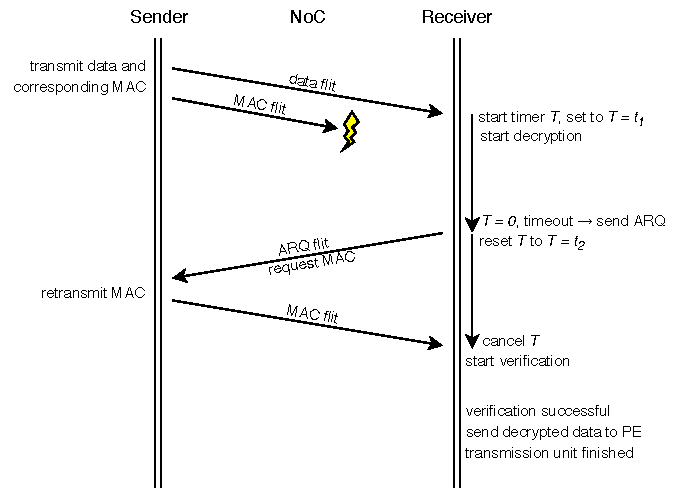
\includegraphics[width=0.8\textwidth]{timeout-indauth-uc}
    \caption[Example flow chart for uncoded ind. auth. with timeouts]{Example flow chart for uncoded individual authentication illustrating the communication
    of a single transmission unit between a sender and a receiver. After the \gls{mac} flit is lost in transit, an \gls{arq} is issued due to the
    timeout.}
    \label{fig:timeoutindauthuc}
\end{figure}

\begin{figure}
    \centering
    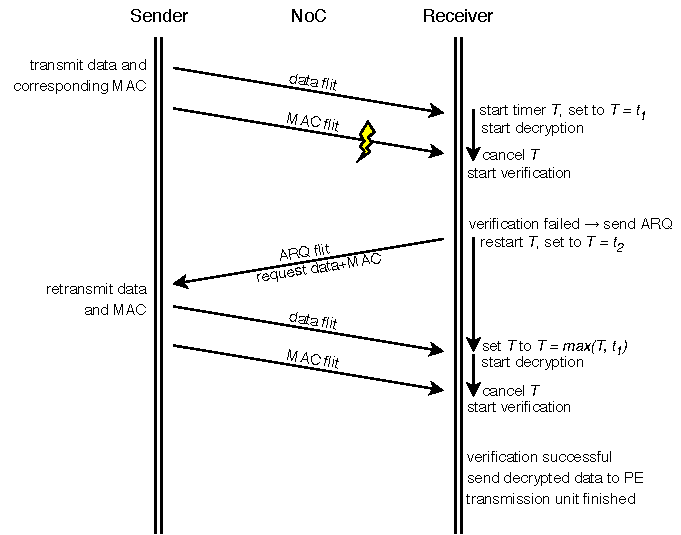
\includegraphics[width=0.8\textwidth]{verification-fail-indauth-uc}
    \caption[Example flow chart for uncoded ind. auth. with integrity breach]{Example flow chart for uncoded individual authentication depicting a
    sender and a receiver communicating a single transmission unit. The \gls{mac} flit is modified in transit, triggering an \gls{arq} to request the
    retransmission of both data and \gls{mac} flit. With the unhindered retransmissions, verification succeeds.}
    \label{fig:verificationfailindauthuc}
\end{figure}

\subsubsection{Network Coded Variant}
\textit{Network coded individual authentication} is the second of the five investigated protocol versions. As the name suggests, it simply adds a
network coding layer to the uncoded variant described above. On the sender side, this layer is inserted after encryption and before authentication,
resulting in the \glspl{mac} being computed over the combinations rather than the uncoded flits. Furthermore, it means that no network coding is
performed over the \gls{mac} flits themselves. Consequently, on the receiver side, decoding needs to be performed before the data flits can be
decrypted. For the verification process, no decoding is required. Figure \vref{fig:protflitdistindauthnc} provides an outside view of the network
interface, while Figure \vref{fig:protchartindauthnc} shows the internal steps.

\begin{figure}
    \centering
    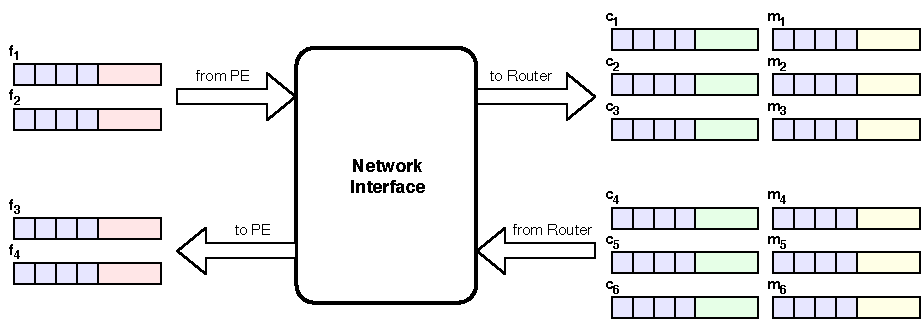
\includegraphics[width=\textwidth]{protocol-flit-distributions-indauth-nc}
    \caption[Network coded ind. auth., outside view]{Outside view of the network interface for network coded individual authentication (G2C3). The
    processing of one transmission unit is depicted for both sending and receiving. For sending, the unencrypted flits $f_1$ and $f_2$ form a
    generation, resulting in the encrypted combinations $c_1$, $c_2$, $c_3$, and their corresponding \gls{mac} flits $m_1$, $m_2$, and $m_3$ being
    injected into the network. For receiving, the arrival of the encrypted combinations $c_4$, $c_5$, $c_6$, and their \glspl{mac} $m_4$, $m_5$, and
    $m_6$ results in the decoded and decrypted flits $f_3$ and $f_4$ being sent to the processing element.}
    \label{fig:protflitdistindauthnc}
\end{figure}

\begin{figure}
    \centering
    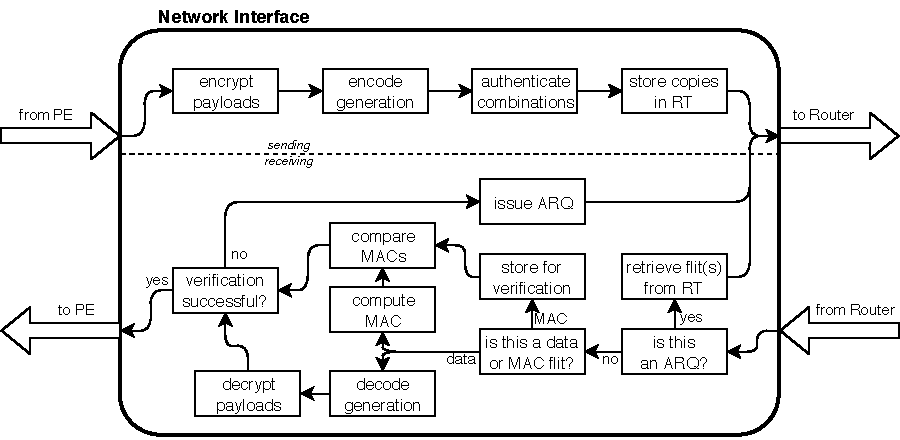
\includegraphics[width=\textwidth]{protocol-chart-indauth-nc}
    \caption[Network coded ind. auth., detailed procedure]{The steps performed by the network interface when processing flits in the network coded
    individual authentication protocol. The upper part of the chart illustrates the sending algorithm, while the lower part depicts the procedure for
    handling arrivals from the network.}
    \label{fig:protchartindauthnc}
\end{figure}
% TODO: say in caption how many flits are needed and are output at coding steps

This amounts to the following procedure for sending flits to the network (upper part of Figure \ref{fig:protchartindauthnc}):
\begin{enumerate}
    \item \textbf{Encrypt payload.} This is precisely the same step as in uncoded individual authentication.
    \item \textbf{Encode generation.} At this stage, the added network coding layer comes in. Incoming flits are buffered in this component until two
        with the same destination are available. Subsequently, network coding is applied to them, resulting in either three (G2C3) or four (G2C4)
        combinations. The used \glspl{gev} and a new generation ID\footnote{The same generation ID is assigned to all combinations.} are stored in
        their designated header fields. The combinations are then passed to the next step; the original flits are not sent out.
    \item \textbf{Authenticate combinations.} The authentication procedure is virtually same as for uncoded individual authentication. The only
        difference is that the \glspl{mac} are computed over combinations rather than uncoded flits (see Figure \vref{fig:computecombinationmac}
        for a visualization of the algorithm)\footnote{Combinations and their \gls{mac} flits are linked by containing the same \gls{gev} value in
        addition to having the same generation ID.}. Apart from that, each incoming combination is individually authenticated with a dedicated \gls{mac}
        flit.
    \item \textbf{Store copies in retransmission buffer.} Unchanged from the uncoded protocol variant, a copy of each flit (combinations and
        \glspl{mac} alike) is stored in the retransmission buffer to facilitate \gls{arq} answers.
\end{enumerate}
\vspace{0.5\baselineskip}

\begin{figure}
    \centering
    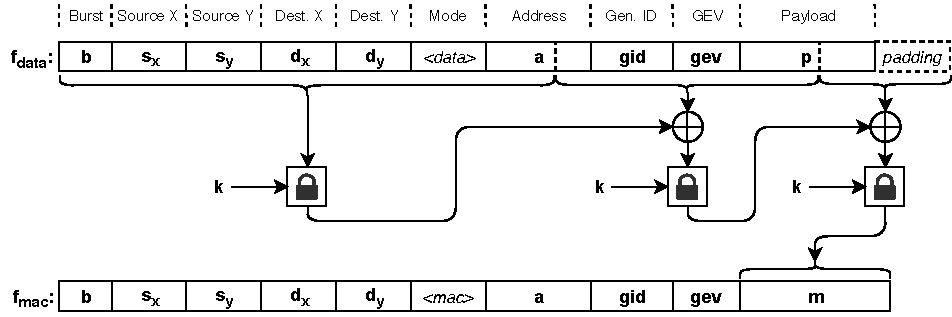
\includegraphics[width=\textwidth]{compute-combination-mac}
    \caption[CBC-MAC algorithm applied to a network coded flit]{The \gls{cbcmac} algorithm applied to a network coded flit. The flit is divided into three
    64-bit blocks, with the last one padded. A \gls{mac} is then computed using \gls{cbcmac} and inserted into the payload of a new flit.}
    \label{fig:computecombinationmac}
\end{figure}

The following processing steps are performed for flits arriving from the network (lower portion of Figure \ref{fig:protchartindauthnc}):
\begin{enumerate}
    \item \textbf{\Gls{arq} handling.} The same procedure as in uncoded individual authentication is performed here.
    \item \textbf{Storing \gls{mac} flits.} Once more, the same actions as in uncoded individual authentication are executed.
    \item \textbf{Processing data flits.} At this point, the protocol starts to differ. As before, the data flit is duplicated, with one copy being
        used to compute its \gls{mac}. The other copy, however, cannot be decrypted yet because the flits are encoded. Hence, it is buffered until two
        flits from the same generation are available, which are thereupon decoded. Afterwards, the resulting flits are decrypted as usual.
    \item \textbf{Verification.} This step is similar to its counterpart in uncoded individual authentication, but not exactly the same. As there are
        multiple verifications required for each transmission unit (one per combination used for decoding), all of them have to succeed. Otherwise, both of the decoded
        and decypted flits for the affected generation must be discarded; a corruption in one of the combinations results in an incorrect decoding. If
        possible, it is retried with a different set of combinations for which the integrity checks have not failed. Once all verifications for the
        combinations used to decode and decrypt the generation have succeeded, the obtained data flits are sent to the processing element.
\end{enumerate}
\vspace{0.5\baselineskip}

\Glspl{arq} are issued for failing integrity checks or when timeouts occur, as illustrated in Figure \vref{fig:timeoutindauthnc}.

\begin{figure}
    \centering
    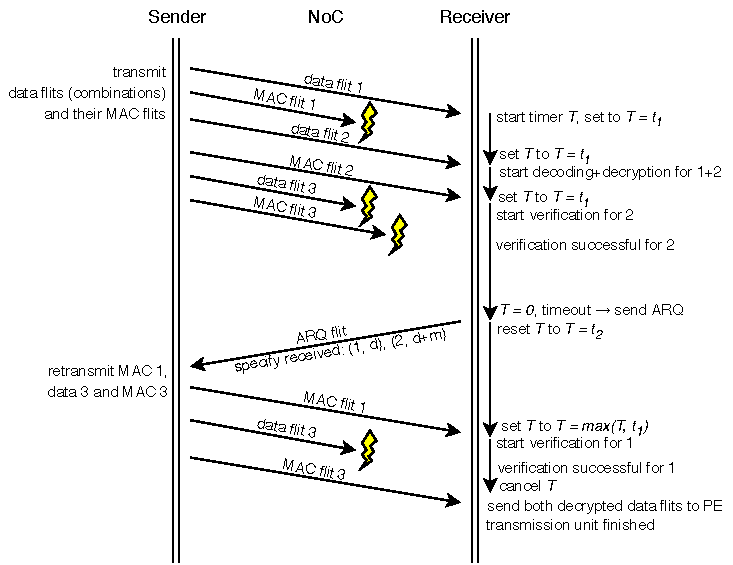
\includegraphics[width=0.8\textwidth]{timeout-indauth-nc}
    \caption[Example flow chart for network coded ind. auth. with many losses]{Example flow chart for network coded individual authentication showing
    a sender and a receiver attempting to communicate a single transmission unit. After half the flits are lost in transit, a timeout occurs. Since
    the receiver does not know the \gls{gev} of the third data/\gls{mac} pair, the subsequent \gls{arq} specifies which flits have already arrived.
    The sender then resends the remaining flits. Even though the third data flit is lost again, the successful arrival of \gls{mac} flit 1 suffices to
    flawlessly process the generation.}
    \label{fig:timeoutindauthnc}
\end{figure}

\subsection{Interwoven Authentication}\label{subsec:intauth}
\subsubsection{Uncoded Variant}
The third scheme in the protocol repertoire is \textit{uncoded interwoven authentication}. Just like the first approach presented in the previous
section (uncoded individual authentication), it facilitates encryption and authentication of the transmitted information. While overall providing the
same features, the key difference lies in the way that flits are authenticated and how this information is consolidated in the flits for transmission.
The goal is to have the data and its authentication information within the same flit to allow receivers to immediately begin the verification process
upon its arrival. However, since the payload size is still limited to 64 bit, a \gls{mac} cannot simply be appended to the data. The implemented
solution is to split the payload in the middle after encryption and moving the second half to a new flit (with the same header fields). Consequently,
both flits contain 32 bit of data and have another 32 bit available for the authentication information. Since they both have the same flit ID to link
them together, the mode field is used to distinguish them (by setting different values for the first and second split, respectively). Figures
\ref{fig:protflitdistintauthuc} and \ref{fig:protchartintauthuc} outline the workings of the network interface for this version of the protocol.

\begin{figure}
    \centering
    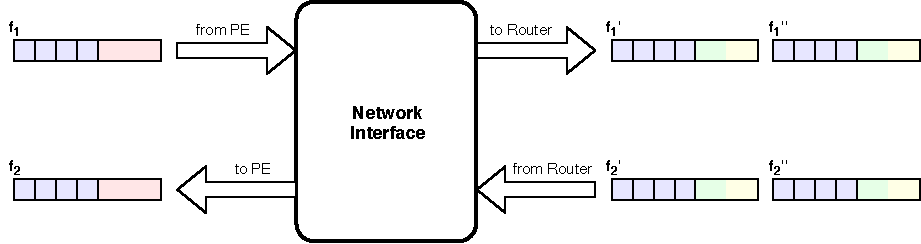
\includegraphics[width=\textwidth]{protocol-flit-distributions-intauth-uc}
    \caption[Uncoded int. auth., outside view]{Outside view of the network interface for uncoded interwoven authentication. The processing of one
    transmission unit is depicted for both sending and receiving. For sending, the unencrypted flit $f_1$ results in the interwoven flits $f_1'$ and
    $f_1''$, each containing encrypted data and their authcode. For receiving, the arrival of the interwoven flits $f_2'$ and $f_2''$ results in the
    merged and decrypted flit $f_2$ being sent to the processing element.}
    \label{fig:protflitdistintauthuc}
\end{figure}

\begin{figure}
    \centering
    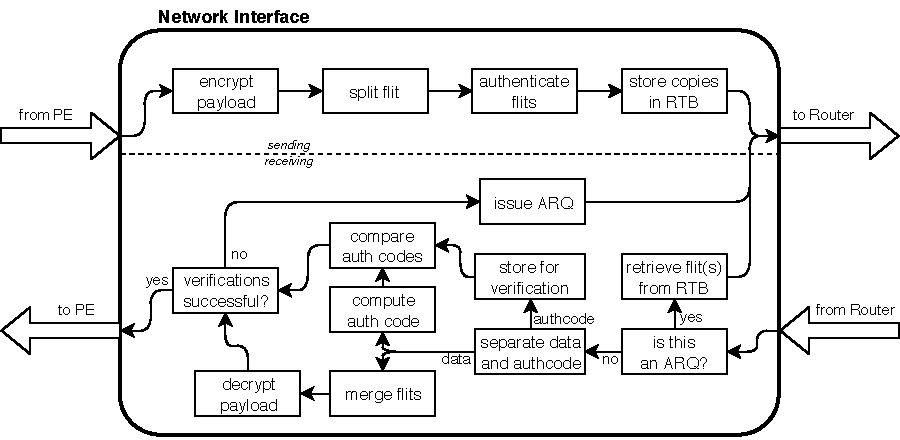
\includegraphics[width=\textwidth]{protocol-chart-intauth-uc}
    \caption[Uncoded int. auth., detailed procedure]{The steps performed by the network interface when processing flits in the uncoded interwoven
    authentication protocol. The upper part of the chart illustrates the sending algorithm, while the lower part depicts the procedure for handling
    arrivals from the network.}
    \label{fig:protchartintauthuc}
\end{figure}

A normal \gls{mac}, as used in individual authentication, has a size of 64 bit by design of the cipher. Thus, the authentication scheme has to be
adapted. A different type of authentication code (called \textit{authcode} in this thesis) provides the solution
\cites{simmons94cryptology}{moriam18activeattackers}. The key idea is to first compute a \gls{mac} as before, but then use it
as a key to create an authcode of half its size (i.e., 32 bit -- precisely the number of available bits). Each bit of the authcode is computed
with two key bits and one bit from the data part of the payload. The pattern is given in Table \vref{tab:authcodes} and the full process
is elucidated in Figure \vref{fig:computeauthcodeuc}. The interweavement of data and authcodes within the same flit is the eponymous characteristic
of this protocol variant.

\begin{table}
    \centering
    \begin{tabulary}{\textwidth}{CC||C|C|C|C}
                                  &    & \multicolumn{4}{c}{key bits} \\
                                  &    & 00 & 01 & 10 & 11 \\\hhline{==#=|=|=|=}
        \multirow{2}{=}{data bit} &  0 &  0 &  0 &  1 &  1 \\\cline{2-6}
                                  &  1 &  0 &  1 &  0 &  1
    \end{tabulary}
    \caption[Bit pattern for the computation of authcodes]{The bit patterns employed when authcodes are computed. One data bit and two key bits
    determine one bit of the authcode \cite[cf.][3]{moriam18activeattackers}.}
    \label{tab:authcodes}
\end{table}

\begin{figure}
    \centering
    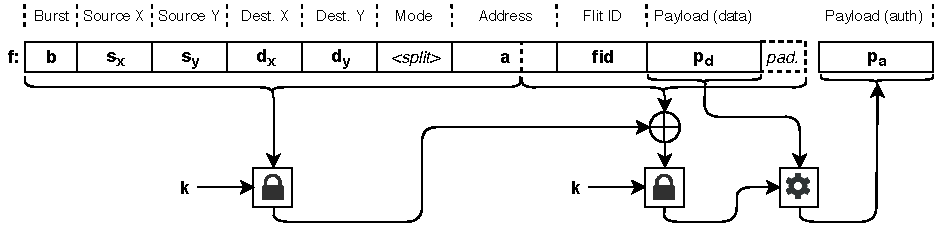
\includegraphics[width=\textwidth]{compute-authcode-uc}
    \caption[Computation of authcodes with CBC-MAC]{Computation of an authcode with \gls{cbcmac}. To compute the intermediate key, \gls{cbcmac} is
    applied to the header fields and the data part of the payload. With a size of 109 bit (or 117 for network coded flits), the input fits into two
    blocks. The padding added to fill the second block is not part of the flit. The intermediate key is then used to compute the actual authcode: the
    cogwheel corresponds to the function defined by Table \ref{tab:authcodes}. The result is stored in the rightmost 32 bit of the flit.}
    \label{fig:computeauthcodeuc}
\end{figure}

Sending a flit from the processing element to the network is achieved by the following course of action (upper part of Figure \ref{fig:protchartintauthuc}):
\begin{enumerate}
    \item \textbf{Encrypt payload.} The encryption process does not differ from uncoded individual authentication.
    \item \textbf{Split flit.} This step is unique to interwoven authentication. As described above, a new flit with the same header values is created
        and the payload is divided among the two flits. Afterwards, one contains the first 32 bit of the payload, while the other holds the last 32
        bit.
    \item \textbf{Authenticate flits.} Each flit is authenticated by computing its authcode, which is then appended to the encrypted data. The 32 data
        bits and the 32 authcode bits form the full payload. In contrast to individual authentication, no additional \gls{mac} flits are generated.
    \item \textbf{Store copies in retransmission buffer.} As usual, a copy of each flit is stored to facilitate retransmissions. This step does not
        differ from the other protocol versions.
\end{enumerate}
\vspace{0.5\baselineskip}

Flits incoming from the network are processed as follows (lower portion of Figure \ref{fig:protchartintauthuc}):
\begin{enumerate}
    \item \textbf{\Gls{arq} handling.} This is the same procedure as in uncoded individual authentication.
    \item \textbf{Separate data and authcode.} The authcode contained in the flit is stored for the imminent integrity check, similar to the
        \gls{mac} flits from the other protocol variants. The remainder of the flit (i.e., the header fields and the 32 bit data part of the payload)
        is duplicated, with one copy being used to compute the verification authcode and the other being buffered for decryption.
    \item \textbf{Merging and decrypting.} Since the sender splits all flits after encryption, both halves are required in order to perform
        decryption. Thus, the flit is buffered as mentioned above until its counterpart arrives. Then, the payload is merged back into a single flit,
        which is subsequently decrypted.
    \item \textbf{Verification.} Once the receiver has computed its own authcode, it is compared with the one contained within the flit. Naturally,
        the integrity check fails should they diverge. If the flit was already decrypted (i.e., the other part of the split has already arrived), the
        result has to be discarded. Once the integrity of both parts is guaranteed, the merged and decrypted flit is sent to the processing element.
\end{enumerate}
\vspace{0.5\baselineskip}

As usual, \glspl{arq} are issued for unsuccessful verifications and timeouts. In contrast to individual authentication, a failed integrity check only
necessitates the retransmission of a single flit.

\subsubsection{Network Coded Variant}
The fourth variation of the protocol adds a network coding layer to interwoven authentication and is thus called \textit{network coded interwoven
authentication}. After an encrypted flit has been split, the two resulting flits form the generation required for network coding. Since their payloads
each contain only 32 bit, the combinations' payloads also just hold 32 bit of encoded data. This leaves the remaining 32 bit for the authcode, which is
computed for each combination using the same algorithm as in uncoded interwoven authentication\footnote{Although network coding introduces the
additional \gls{gev} header field to the flits, the input for the \gls{cbcmac} part of the algorithm, being 117 bit in size, still fits into two
blocks.}. On the receiver side, the network coding layer introduces an additional decoding step before the flits are merged and decrypted. As before,
an outside view of the network interface is given in Figure \vref{fig:protflitdistintauthnc}, while the internal procedures are outlined in Figure
\vref{fig:protchartintauthnc}.

\begin{figure}
    \centering
    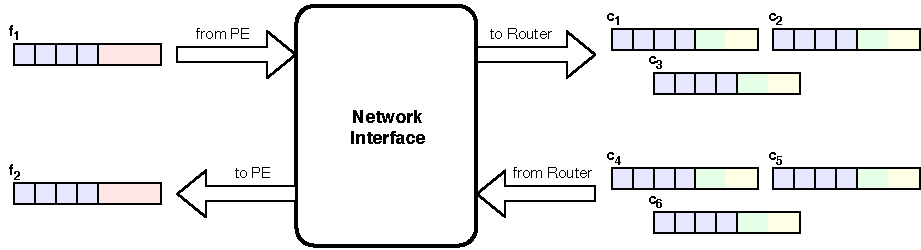
\includegraphics[width=\textwidth]{protocol-flit-distributions-intauth-nc}
    \caption[Network coded int. auth., outside view]{Outside view of the network interface for network coded interwoven authentication (G2C3). The
    processing of one transmission unit is depicted for both sending and receiving. For sending, the unencrypted flit $f_1$ results in the interwoven
    combinations $c_1$, $c_2$, and $c_3$, each containing encrypted, encoded data and their authcode. For receiving, the arrival of the interwoven
    combinations $c_4$, $c_5$, and $c_6$ results in the decoded, merged, and decrypted flit $f_2$ being sent to the processing element.}
    \label{fig:protflitdistintauthnc}
\end{figure}

\begin{figure}
    \centering
    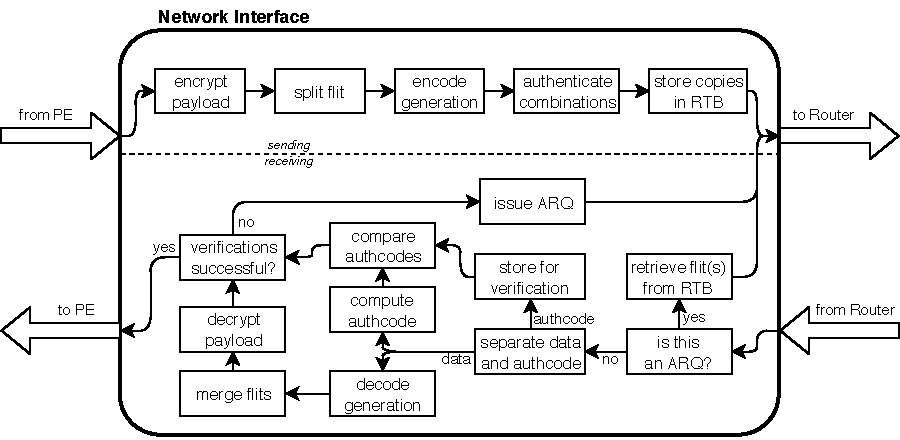
\includegraphics[width=\textwidth]{protocol-chart-intauth-nc}
    \caption[Network coded int. auth., detailed procedure]{The steps performed by the network interface when processing flits in the network coded
    interwoven authentication protocol. The upper part of the chart illustrates the sending algorithm, while the lower part depicts the procedure for
    handling arrivals from the network.}
    \label{fig:protchartintauthnc}
\end{figure}

The following steps are implemented on the sender side (upper part of Figure \ref{fig:protchartintauthnc}):
\begin{enumerate}
    \item \textbf{Encrypt payload.} As per usual, this is the first piece of the sending process and does not differ from the other protocol variants.
    \item \textbf{Split flit.} The same procedure as in uncoded interwoven authentication is applied here.
    \item \textbf{Encode generation.} As described above, the flits resulting from the split form a generation for network coding. The encoding
        algorithm is the same as in network coded individual authentication.
    \item \textbf{Authenticate combinations.} For each combination, an authcode is computed in the same manner as in uncoded interwoven
        authentication. It is inserted into the last 32 bit of the payload, which are not occupied by encoded data.
    \item \textbf{Store copies in retransmission buffer.} As in all protocol variants, a copy of each flit that is leaving for the network is retained
        to answer potential future \glspl{arq}.
\end{enumerate}
\vspace{0.5\baselineskip}

The network interface employs the following procedures to handle flits arriving from the network (lower portion of Figure
\ref{fig:protchartintauthnc}):
\begin{enumerate}
    \item \textbf{\Gls{arq} handling.} There is no change from the uncoded variant of this step.
    \item \textbf{Separate data and authcode.} Similar to the uncoded version, the authcode is separated from the combination and stored for the
        imminent verification process. The remainder of the flit is duplicated, with one copy being used to compute its authcode. The other copy is
        buffered, but for decoding instead of decryption.
    \item \textbf{Decoding, merging, and decrypting.} Comparable to network coded individual authentication, the decoding process cannot start until
        two flits from the same generation are available. Once they have arrived, the combinations are decoded. The resulting flits are subsequently
        merged and decrypted.
    \item \textbf{Verification.} Once the computed authcode is available, it is compared against the stored one. A divergence indicates a corruption
        in the flit. If decoding was already performed with the affected flit, the result must be discarded since its integrity cannot be assured. If
        the verification process succeeds for all combinations that are used for decoding, the decrypted flit is sent to the processing element once
        it is available.
\end{enumerate}
\vspace{0.5\baselineskip}

As in the uncoded variant, \glspl{arq} only need to request one flit in the event of an integrity breach. For timeouts, the same rules as for the
other variants apply. An example is given in Figure \vref{fig:verificationfailintauthnc}.

\begin{figure}
    \centering
    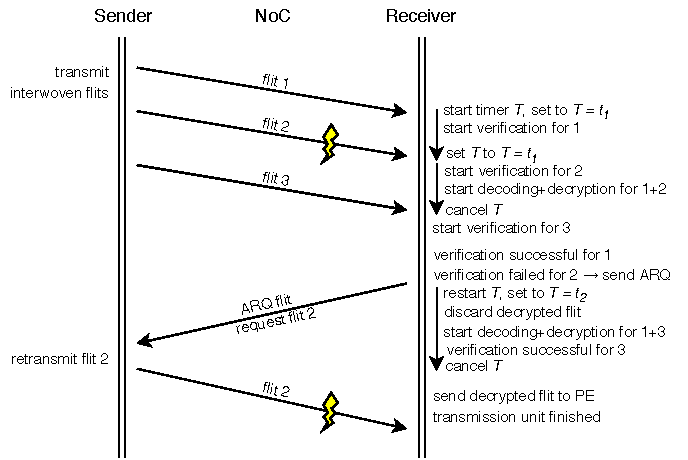
\includegraphics[width=0.8\textwidth]{verification-fail-intauth-nc}
    \caption[Example flow chart for network coded int. auth. with integrity breach]{Example flow chart for network coded interwoven authentication
    with a sender and a receiver attempting to communicate a single transmission unit. The second flit is modified in transit, triggering an \gls{arq}
    to request its retransmission. Furthermore, the already decoded, merged, and decrypted flit has to be discarded and the process is retried with
    flits 1 and 3. With the integrity check for flit 3 succeeding, flit 2 becomes obsolete and the modification of its retransmission does not
    matter.}
    \label{fig:verificationfailintauthnc}
\end{figure}

\subsection{Full-Generation Authentication}\label{subsec:genauth}
The fifth and final protocol variant is \textit{full-generation authentication}. In contrast to individual and interwoven authentication, it only
exists in a network coded form because it presumes the existance of generations for its authentication scheme.

Every generation is authenticated in its entirety, i.e., one \gls{mac} flit is created for the whole generation. A key difference to all other
protocol variants is the order of network coding and authentication: here, the \gls{mac} is computed over the uncoded flits instead of the
combinations. Ordering it the other way around would nullify the main benefit of network coding: partial flit loss (or corruption) would no longer be
tolerable. With a single \gls{mac} being computed over all combinations, each one would be required to arrive at the destination to render verification
possible, and a single corrupted combination would breach the integrity of the whole generation. Thus, the \gls{mac} is computed over the uncoded
flits before encoding. The \gls{mac} is transmitted via a separate flit (as in individual authentication) and is not a part of the encoding process.
Figure \vref{fig:protflitdistgenauth} depicts the protocol from an outside point of view, while Figure \vref{fig:protchartgenauth} details the
individual steps.

\begin{figure}
    \centering
    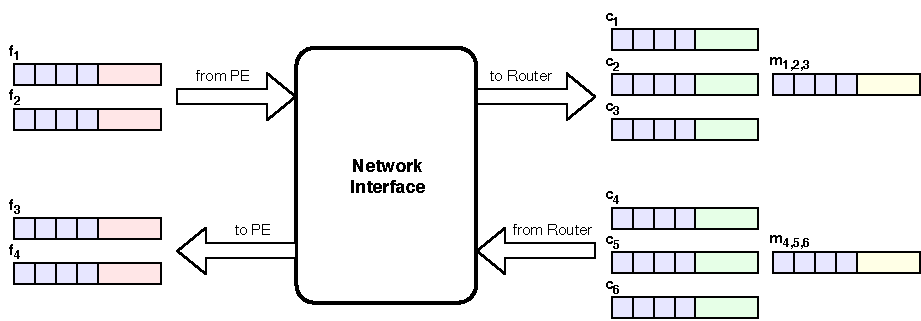
\includegraphics[width=\textwidth]{protocol-flit-distributions-genauth}
    \caption[Full-gen. auth., outside view]{Outside view of the network interface for full-generation authentication (G2C3). The processing of one
    transmission unit is depicted for both sending and receiving. For sending, the unencrypted flits $f_1$ and $f_2$ form a generation, resulting in
    the \gls{mac} flit $m_{1,2,3}$ and the combinations $c_1$, $c_2$, and $c_3$ being injected into the network. For receiving, the arrival of the
    combinations $c_4$, $c_5$, $c_6$, and the generation \gls{mac} $m_{4,5,6}$ results in the decoded and decrypted flits $f_3$ and $f_4$.}
    \label{fig:protflitdistgenauth}
\end{figure}

\begin{figure}
    \centering
    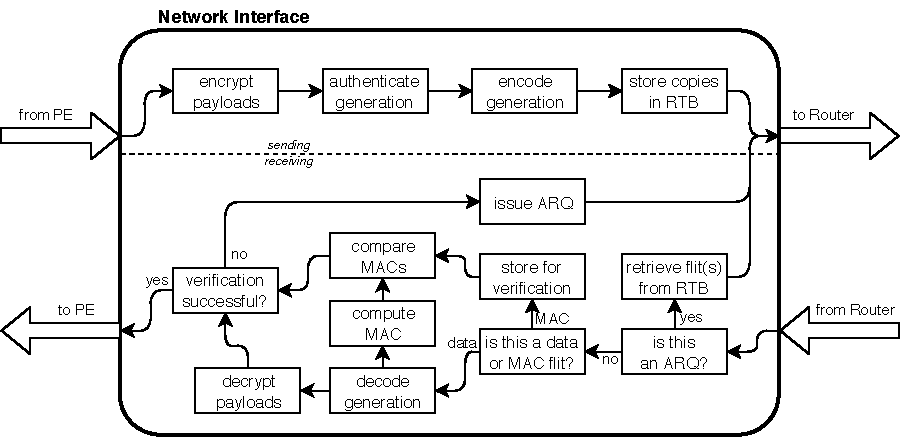
\includegraphics[width=\textwidth]{protocol-chart-genauth}
    \caption[Full-gen. auth., detailed procedure]{The steps performed by the network interface when processing flits in the full-generation
    authentication protocol. The upper part of the chart illustrates the sending algorithm, while the lower part depicts the procedure for handling
    arrivals from the network.}
    \label{fig:protchartgenauth}
\end{figure}

On the sender side, the following procedure is applied to the flits (upper part of Figure \ref{fig:protchartgenauth}):
\begin{enumerate}
    \item \textbf{Encrypt payload.} This step is the same as in the other protocol versions.
    \item \textbf{Authenticate generation.} As explained above, the \gls{mac} is computed over the uncoded flits of a generation. Flits that arrive
        here are buffered until two with the same destination are available. Subsequently, a single \gls{mac} is computed over both of them and placed
        in a new, dedicated flit with the same header fields (except for the mode, which is set to the value indicating a \gls{mac}). The underlying
        algorithm is \gls{cbcmac} as usual, but with a total of five input blocks since two data flits are processed at once (with a total size of 298
        bit). Figure \vref{fig:computegenerationmac} illustrates this step.
    \item \textbf{Encode generation.} The data flits that have just been authenticated are now encoded. The algorithm is the same as in network coded
        individual authentication, with one exception: any \gls{mac} flits that arrive at this component are passed on unchanged.
    \item \textbf{Store copies in retransmission buffer.} A copy of each flit is kept to answer \glspl{arq} should the need arise. The original flits
        are sent to the network.
\end{enumerate}
\vspace{0.5\baselineskip}

\begin{figure}
    \centering
    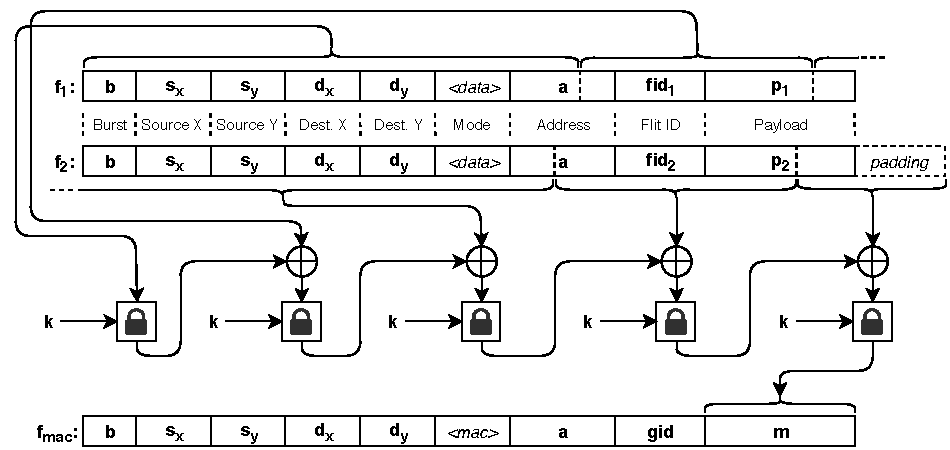
\includegraphics[width=\textwidth]{compute-generation-mac}
    \caption[CBC-MAC algorithm applied to a generation]{The \gls{cbcmac} algorithm applied to a generation (before network coding). The two flits are
    concatenated, resulting in a total size of 298 bit and thus five input blocks. The last block is filled with padding bits. After running the
    algorithm, the computed \gls{mac} is inserted into the payload of a new flit.}
    \label{fig:computegenerationmac}
\end{figure}

The receiver uses the following course of action (lower portion of Figure \ref{fig:protchartgenauth}):
\begin{enumerate}
    \item \textbf{\Gls{arq} handling.} The treatment of incoming \glspl{arq} is the same as in the other protocol variants described above.
    \item \textbf{Storing \gls{mac} flits.} If a generation's \gls{mac} flit arrives, it is stored for the integrity check as usual.
    \item \textbf{Decoding.} In contrast to all other protocol variants, the combinations need to be decoded before the verification \glspl{mac} can
        be computed. Flits are thus buffered here until two combinations from the same generation are available. Then, the normal decoding process is
        performed.
    \item \textbf{Processing decoded flits.} After decoding, the flits are duplicated. One copy of each is used to compute the \gls{mac} of the
        generation, while the other ones are sent to decryption.
    \item \textbf{Verification.} Once the network interface has computed the verification \gls{mac} and received the transmitted \gls{mac} from the
        network, they are compared as usual. If they are equal, the decrypted flits are intact and thus forwarded to the processing element.
        Otherwise, the received \gls{mac} or one of the combinations used for decoding is corrupted. Consequently, the decrypted flits must be
        discarded. If further combinations are available, decoding and \gls{mac} computation is retried with a different set.
\end{enumerate}
\vspace{0.5\baselineskip}

When a failed integrity check triggers an \gls{arq} issuance, both combinations used in the decoding process in addition to the generation's
\gls{mac} are requested. This is necessary since the receiver cannot know which one of them was modified in transit. Furthermore, \glspl{arq} are
issued on timeouts as per usual.

\section{Routing}
A core aspect of this thesis is the exploration of different routing strategies and their effects on the performance and reliability of
the network. Several routing strategies with different path selection algorithms are investigated. Recalling that the topology of the
\gls{noc} is a 2D mesh, there is a multitude of possible paths to reach a destination from a particular source node. Figure \vref{fig:pathexamples}
illustrates some exemplary ones\footnote{The processing elements and network interfaces are omitted for illustration purposes.}.

\begin{figure}
    \centering
    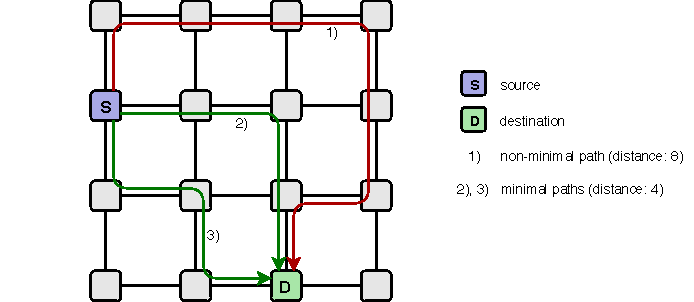
\includegraphics[width=0.9\textwidth]{path-examples}
    \caption[Examples of different paths between two nodes]{Example of different possible paths through a 2D mesh \gls{noc} for a particular source
    and destination node pair. Paths 2 and 3 have the minimal Manhattan distance of 4 hops.}
    \label{fig:pathexamples}
\end{figure}

To narrow down the set of considered paths, only those with a minimal Manhattan distance between source and destination are examined. Consequently, this
leaves only one viable path when the source and destination nodes lie on the same row or column of the mesh. Else, they still have multiple minimal
routes at disposal. The path selection methods described in this section thus only apply to those source-destination node pairs lying on different
rows and columns of the mesh. As the title of this thesis suggests, making use of the full bandwidth of available paths by selecting them
independently for each flit is of particular interest here.

\subsection{Characteristics And Classification}
Routing strategies may be classified according to their properties. The following list and Figure \ref{fig:routingcharacteristics} explain the important
characteristics and the distinctions between them.
\begin{itemize}
    \item \textbf{Oblivious vs. adaptive.} When the source or an intermediate node decides on the next hop of a route, it may take the current
        network state into account. For instance, a congestion detected on the preferred port\footnote{Congestion is detected by inspecting the length
        of the neighboring router's input queue for the appropriate port; if it is full, the link to this router is viewed as congested. The details
        of this process are explained in Section (insert ref here).} may dissuade the router from forwarding the flit in this direction and instead
        use a different port, as long as the resulting route is still minimal. If the network state influences the routing decision, the strategy is
        adaptive. In contrast, an oblivious one does not take the state into consideration. In case of a congestion, forwarding of the flit is delayed
        until the path is available again. The oblivious strategies explored here are \gls{dor} and \gls{romm}, while \gls{dm} and \gls{ramm} are
        adaptive. They are described in Section \ref{subsec:routingstrategies} below.
    \item \textbf{Static vs. dynamic.} A static strategy implies that exactly one fixed, deterministically chosen path exists for each pair of source
        and destination node. A dynamic one entails a path being selected for each flit individually at runtime. Consequently, static strategies are
        always oblivious and adaptive ones are always dynamic. Since the emphasis lies on the usage of multiple paths, the only investigated static
        strategy is \gls{dor}, serving as a baseline for comparison with the other ones.
\end{itemize}
\vspace{0.5\baselineskip}

\begin{figure}
    \centering
    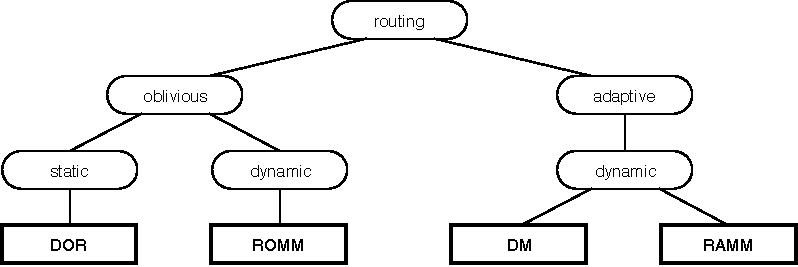
\includegraphics[width=0.8\textwidth]{routing-characteristics}
    \caption[Routing strategies by category]{The evaluated routing strategies categorized by their characteristics.}
    \label{fig:routingcharacteristics}
\end{figure}

The main benefit of dynamic strategies presents itself when used in combination with a network coded protocol. Since each flit is routed individually,
members of the same generation are likely to take diverging paths (as long as source and destination lie on different rows and columns of the
\gls{noc}). Thus, if malicious routers are situated within the rectangle spanned by source and destination, the variety of paths may enable a portion
of the flits to circumvent them, allowing for successful decoding even if the others are modified. Figure \vref{fig:circumventattackers} exemplifies
this scenario with the network coded interwoven authentication protocol.% TODO: mention out of order arrival with dynamic, not possible with static

\begin{figure}
    \centering
    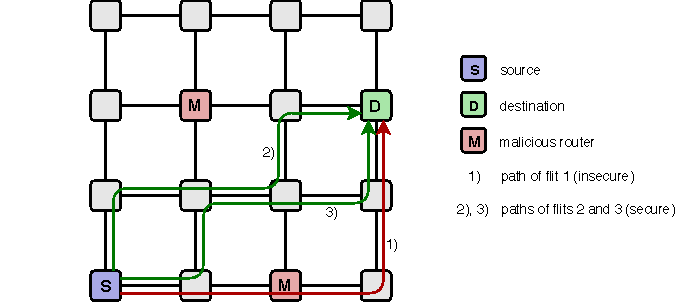
\includegraphics[width=0.9\textwidth]{circumvent-attackers}
    \caption[Example of dynamic routing dodging malicious routers]{Example of a \gls{noc} with two malicious routers and a generation being
    transmitted via the network coded interwoven authentication protocol (G2C3) and dynamic routing. While flit 1 is modified by a malicious router,
    the paths of flits 2 and 3 do not include an attacker, enabling the destination node to successfully decode the generation. With \gls{dor}, every
    flit would use path 1, enabling the malicious router to corrupt all of them.}
    \label{fig:circumventattackers}
\end{figure}

Adaptive strategies enable routers to circumvent congested paths as long as an alternative route is available. Their purpose is to reduce latencies in
saturated networks and produce a more uniform distribution of the traffic over the network.

\subsection{Explored Strategies}\label{subsec:routingstrategies}
\subsubsection{Dimension Order}\label{subsubsec:dor}
\textit{Dimension Order Routing (\gls{dor})}, sometimes referred to as \textit{XY Routing}, is an oblivious, static routing strategy. Flits are first
forwarded along the rows of the mesh (the X dimension) until they arrive at the column that their destination is situated in. Then, they are routed
along this column (the Y dimension) until reaching their target. This is the simplest of the examined strategies and used as a baseline for the
evaluation of the other ones. Exemplary paths are depicted in Figure \ref{fig:allstrategiespaths}a.

Due to its simplicity, this strategy can be implemented in routers without increasing their complexity, and thus their occupied chip area, by a lot.
However, its performance deteriorates considerably under heavy network loads \cite[3]{nesson95romm}. Furthermore, it does not offer the advantages of
multipath routing described above.

\subsubsection{Dynamic Minimal}\label{subsubsec:dm}
The second strategy of interest is \textit{Dynamic Minimal Routing (\gls{dm})}. When a router has multiple options for the next hop of a flit, it checks
the congestion status of the viable output ports. In a 2D mesh, at most two directions are allowed in order for the path to remain minimal. If both
are free, one of them is chosen at random. If only one of them is uncongested, it is always selected. In the event of both viable paths being blocked,
the flit is held back until one of them becomes available. These steps are performed by every router along the flit's path. Figure
\ref{fig:allstrategiespaths}b shows a few of the possible paths.

The adaptiveness of this scheme allows for the possibility to dodge saturated areas of the network. Together with the random selections in the
intermediate routers, it facilitates the use of multiple paths for each pair of source and destination node. However, it requires a random number
generator to be integrated into the routers, increasing their hardware complexity.

\subsubsection{Randomized Oblivious Multi-Phase Minimal}\label{subsubsec:romm}
\textit{Randomized Oblivious Multi-Phase Minimal Routing (\gls{romm})} is a class of routing algorithms originally designed as a compromise between
static, minimal and randomized, non-minimal routing \cite[3]{nesson95romm}. The central idea is to have the source select $n$ nodes at random
through which the flit must be routed, essentially dividing the path into multiple independent segments (hence the name \enquote{multi-phase}). To
preserve minimality, each node $i\ |\ i \in [1,n]$ must lie within the rectangle spanned by node $i-1$ and the destination\footnote{For uniformity,
node $0$ is defined as the source node.}. \Gls{dor} is employed to route the flit from node $i-1$ to $i\ |\ i \in [1,n]$ and from $n$ to the
destination. Since \gls{dor} is oblivious and the selection of the intermediate nodes is not influenced by the network state, \gls{romm} is oblivious
as well.

For this thesis, the version with $n = 1$ intermediate nodes is employed. The name \textit{\gls{romm}} will henceforth be used to refer to this
specific algorithm rather than the whole class. In other words, the source chooses one intermediate node from the rectangle spanned by it and
the destination; then \gls{dor} is used for the path from source to intermediate and from intermediate to destination\footnote{As the intermediate
node is selected by the source, this information needs to be transmitted along with the flit to render this strategy possible. This increases the flit
size by 8 bit (4 bit X and 4 bit Y coordinate, see Section \ref{subsec:flitstructure}). To maintain uniformity, the increase is ignored here. The
number of input blocks for the authentication ciphers is not affected; the padding is simply 8 bit shorter.}. An example is given in Figure
\ref{fig:allstrategiespaths}c.

\Gls{romm} provides a middle ground between \gls{dor} and \gls{dm}. Random number generation is still required, but only needs to be performed by the
source instead of every node along the flit's path.

\subsubsection{Randomized Adaptive Multi-Phase Minimal}\label{subsubsec:ramm}
With \gls{romm} providing dynamic routing, but in an oblivious manner, the creation of an adaptive version suggested itself. Thus, \textit{Randomized
Adaptive Multi-Phase Minimal Routing (\gls{ramm})} was designed. It is very similar to \gls{romm} and employs the same approach to select an
intermediate node. However, during the individual phases, \gls{dm} is used instead of \gls{dor} to introduce a certain degree of adaptiveness to the
algorithm. Note that the selection of the intermediate node is still oblivious to the network state. Figure \ref{fig:allstrategiespaths}d depicts an
exemplary path for this strategy.

\begin{figure}
    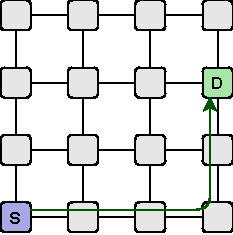
\includegraphics[width=0.22\textwidth]{routing-example-dor}\hfill
    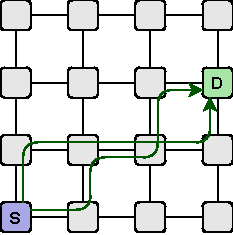
\includegraphics[width=0.22\textwidth]{routing-example-dm}\hfill
    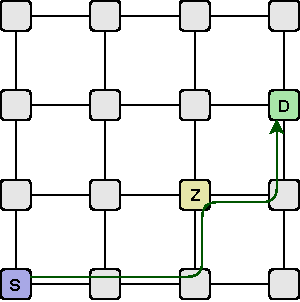
\includegraphics[width=0.22\textwidth]{routing-example-romm}\hfill
    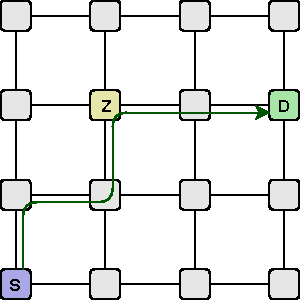
\includegraphics[width=0.22\textwidth]{routing-example-ramm}\\
    \vspace{0.5\baselineskip}
    \begin{footnotesize}
        \hspace*{0.08\textwidth}\textbf{(a)}\hfill\textbf{(b)}\hfill\textbf{(c)}\hfill\textbf{(d)}\hspace*{0.08\textwidth}
    \end{footnotesize}
    \caption[Exemplary paths for the examined routing strategies]{Exemplary paths for each of the examined routing strategies: (a) \gls{dor}, (b)
    \gls{dm}, (c) \gls{romm}, (d) \gls{ramm}. The nodes labeled with Z represent the randomly selected intermediate nodes for the multi-phase
    strategies.}
    \label{fig:allstrategiespaths}
\end{figure}

% TODO: table comparing the routing strategies (adaptive yes/no, static yes/no, out-of-order arrival possible yes/no, ...)
